\subsection{Triển khai mạng blockchain qua Chainlaunch}

Phần này trình bày quy trình triển khai hạ tầng mạng Hyperledger Fabric phục vụ hệ thống bỏ phiếu điện tử, sử dụng nền tảng Chainlaunch để tự động hóa và quản trị toàn bộ vòng đời các node mạng.

\subsubsection{Thiết kế kiến trúc mạng}

Hệ thống bầu cử điện tử yêu cầu mức độ sẵn sàng cao và khả năng chống lỗi tốt. Mạng blockchain được xây dựng trên nền tảng Hyperledger Fabric với định danh tổ chức \pkg{org1msp} và kênh truyền thông \pkg{votechannel}, hạ tầng được phân tách thành 5 node cốt lõi:

\begin{itemize}
    \item \textbf{Thành phần đồng thuận (Ordering Service):} Gồm 3 node Orderer cấu hình theo thuật toán Raft (\pkg{orderer0-org1msp}, \pkg{orderer1-org1msp}, \pkg{orderer2-org1msp}) lần lượt trên cổng 9000, 9100 và 9200, đảm bảo tính toàn vẹn dữ liệu và bảo đảm thứ tự giao dịch, tạo khối và duy trì khả năng chịu lỗi của cụm đồng thuận theo mô hình chịu lỗi (\textit{fault-tolerant}).

    \item \textbf{Thành phần lưu trữ và xác thực (Peer Nodes):} Gồm 2 node (\pkg{peer0-org1msp} trên cổng 7000 và \pkg{peer1-org1msp} trên cổng 7100) đóng vai trò lưu trữ bản sao sổ cái (Ledger) và thực thi hợp đồng thông minh.
\end{itemize}

\begin{figure}[H]
    \centering
    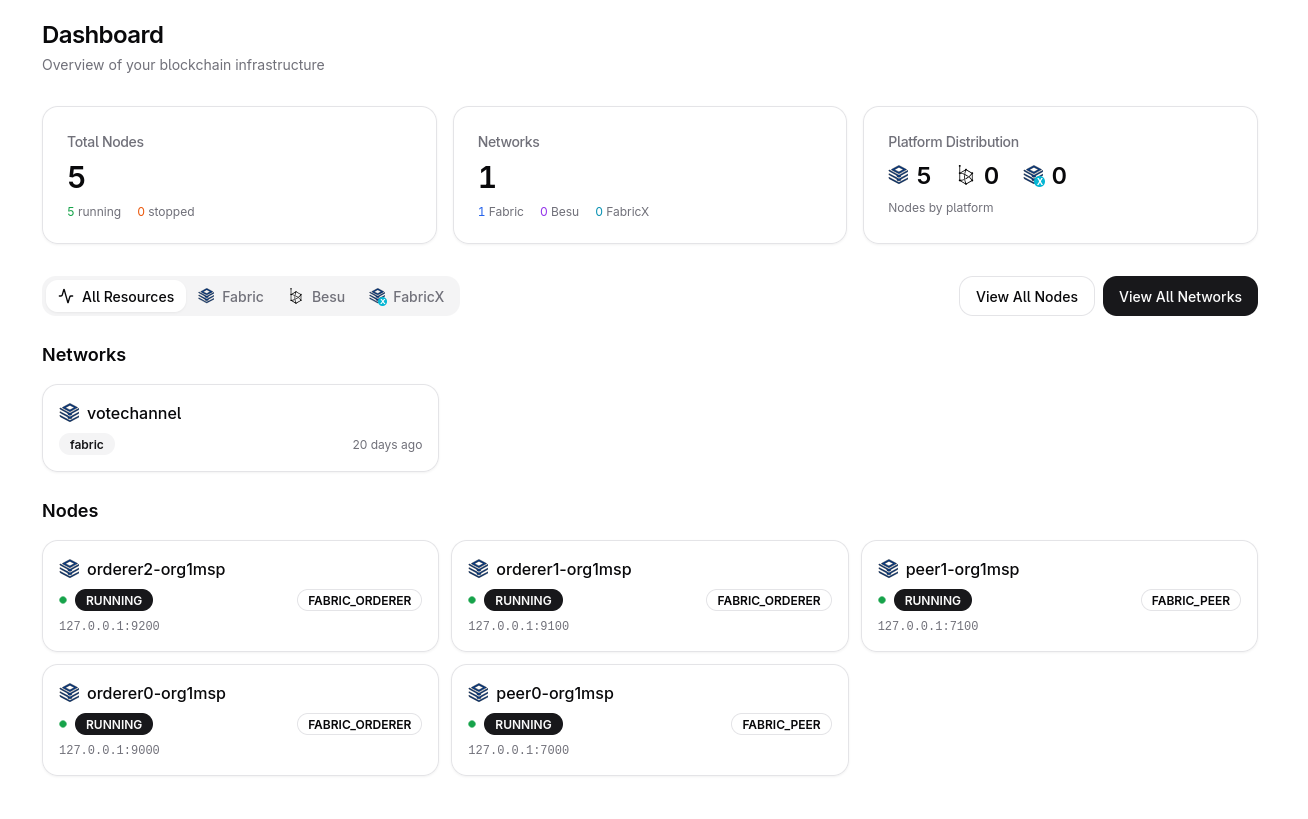
\includegraphics[width=\textwidth, keepaspectratio]{Figures/Chainlaunch-dashboard.png}
    \caption{Giao diện dashboard quản lý mạng blockchain trên nền tảng Chainlaunch}
    \label{fig:chainlaunch-dashboard}
\end{figure}

Hình~\ref{fig:chainlaunch-deploy-all} trình bày toàn bộ trình tự lệnh triển khai theo sáu bước với bộ công cụ giao diện dòng lệnh Chainlaunch CLI .

\begin{figure}[H]
    \centering
    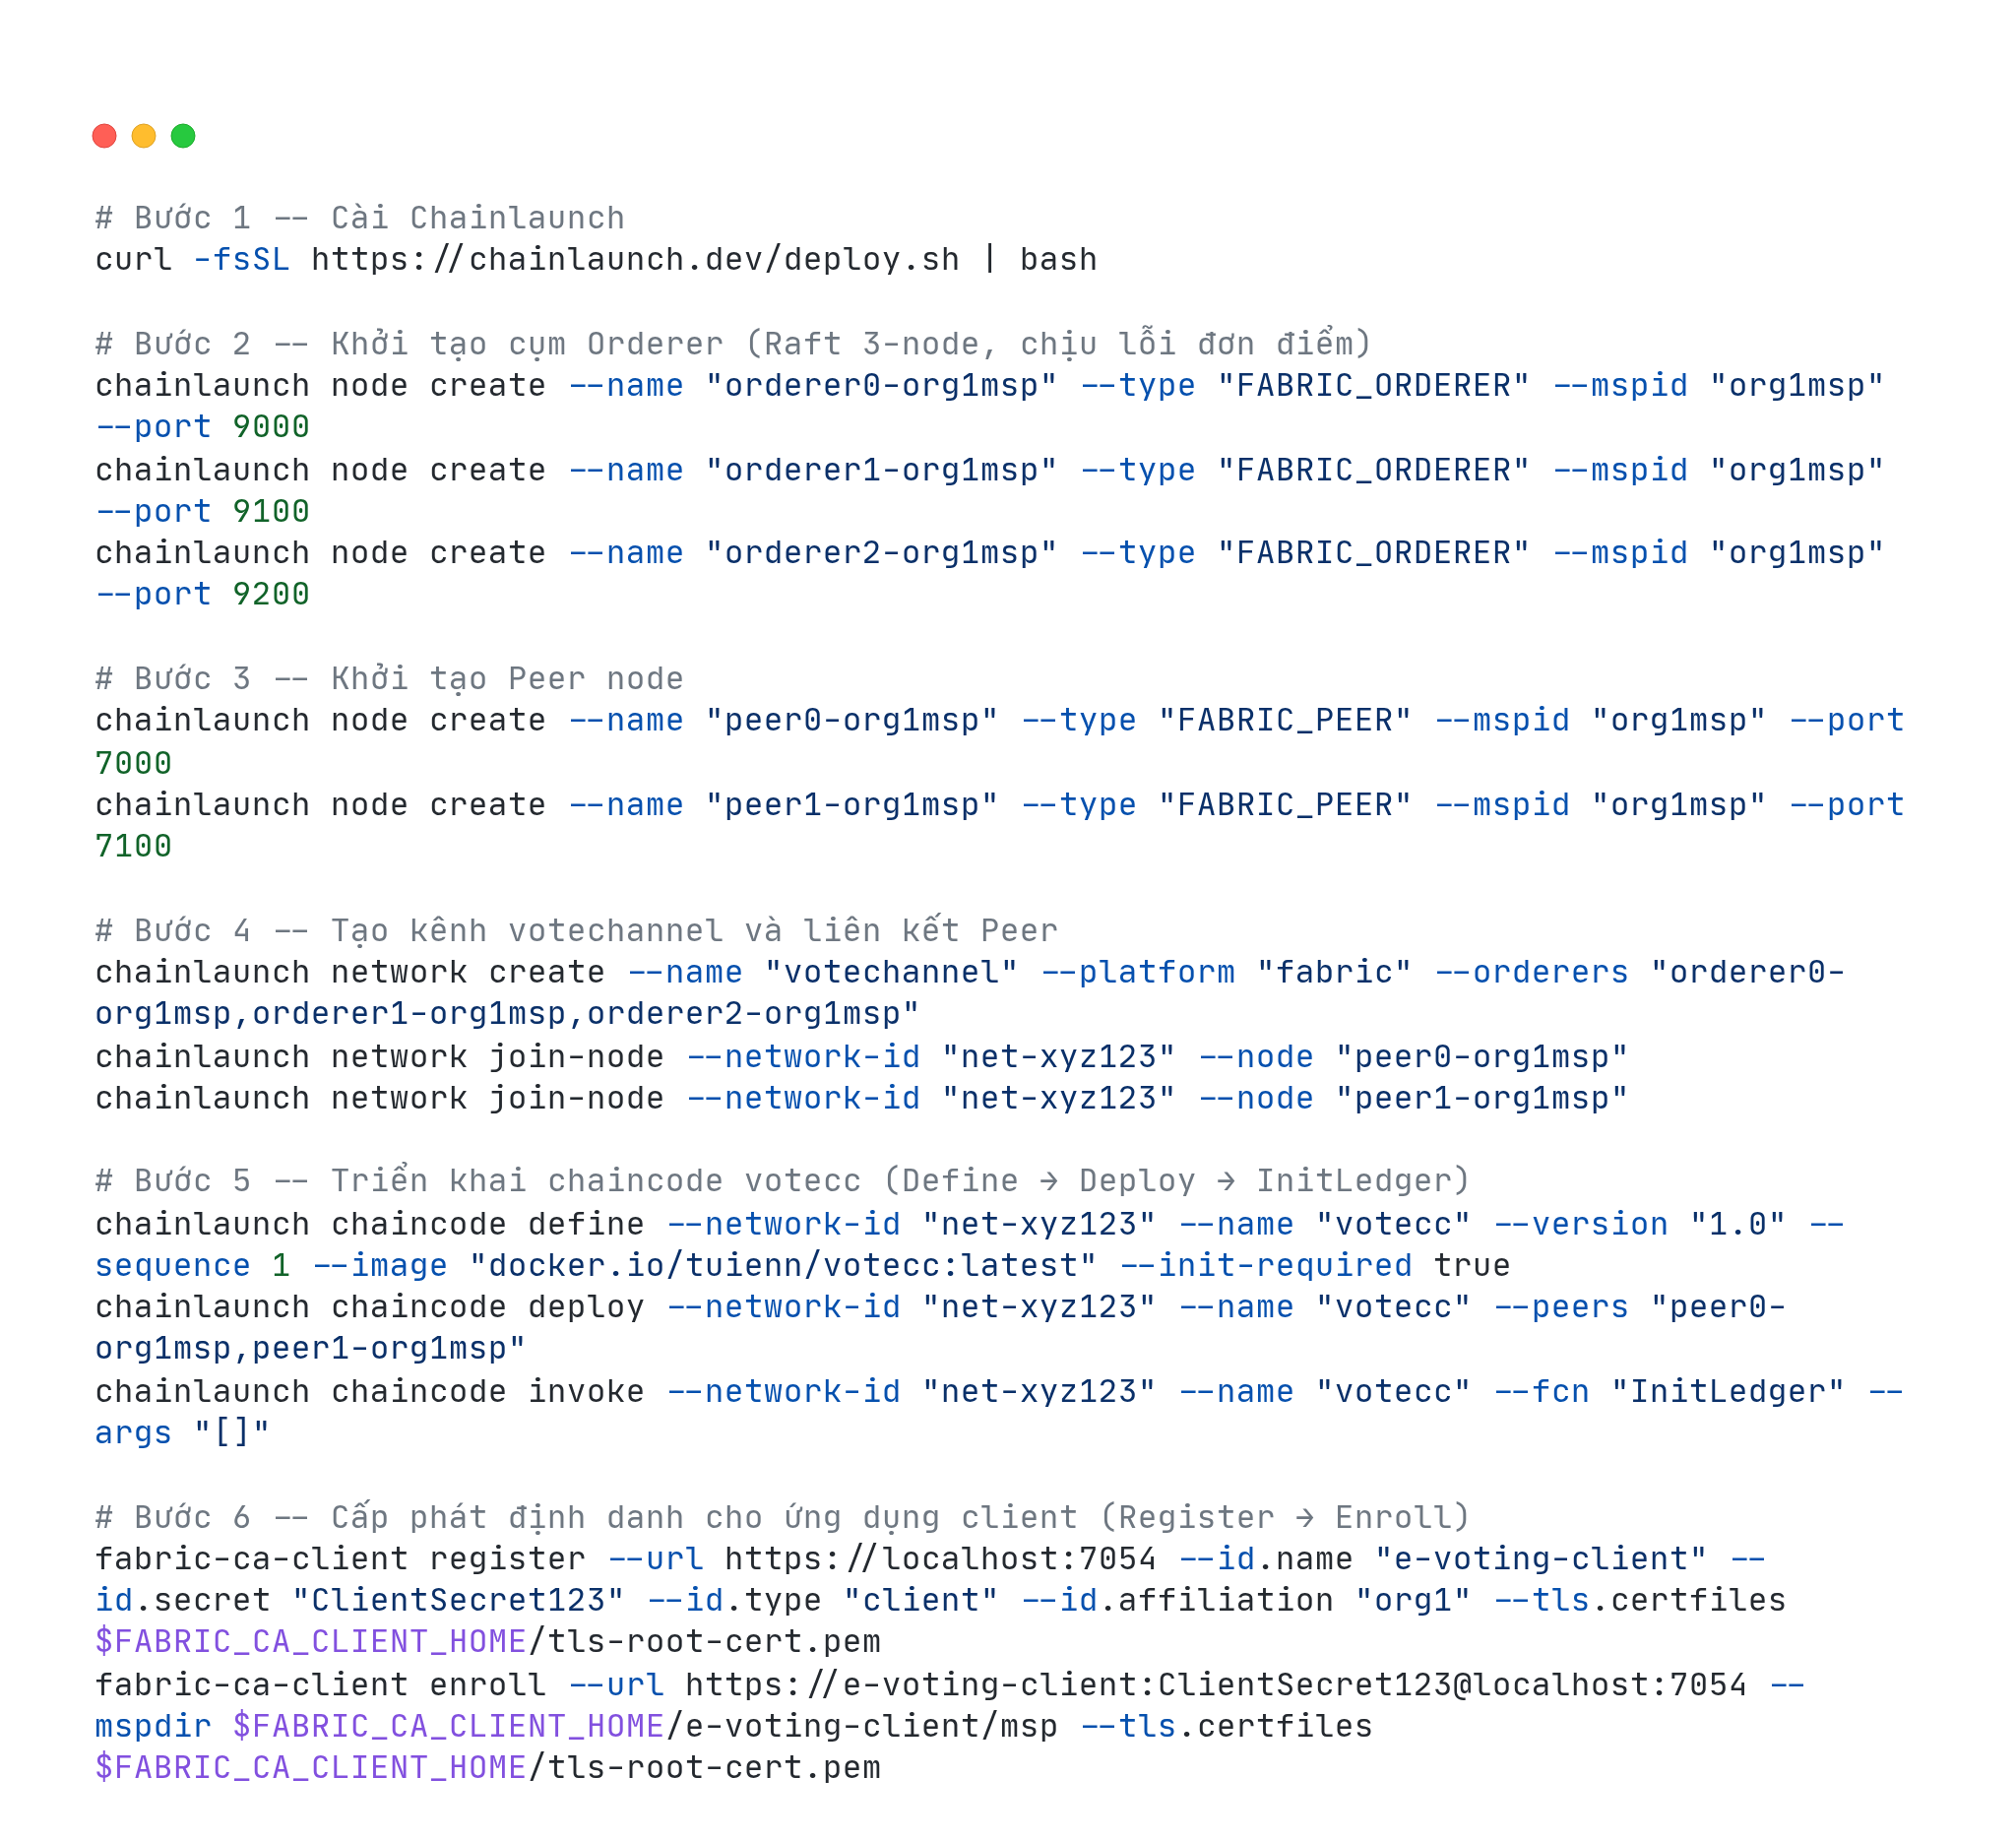
\includegraphics[width=\textwidth, keepaspectratio]{Figures/code/chainlaunch-deploy-all.png}
    \caption{Trình tự lệnh triển khai mạng blockchain e-voting (6 bước)}
    \label{fig:chainlaunch-deploy-all}
\end{figure}

\subsubsection{Khởi tạo các node mạng}

Toàn bộ thao tác khởi tạo tài nguyên mạng được thực hiện tuần tự thông qua Chainlaunch CLI, đảm bảo tính minh bạch và ghi vết đầy đủ vòng đời từng node. Đầu tiên, cụm đồng thuận gồm 3 node Orderer độc lập được kích hoạt nhằm loại bỏ điểm lỗi duy nhất (Single Point of Failure).

Tiếp theo, 2 peer node được khởi tạo, chịu trách nhiệm nhận đề xuất giao dịch bầu chọn từ phía người dùng.

\subsubsection{Thiết lập kênh truyền thông}

Kênh \pkg{votechannel} đóng vai trò là không gian mạng riêng tư, cô lập dữ liệu bầu chọn giữa các thực thể tham gia. Quá trình tạo lập bắt đầu bằng việc liên kết cụm Orderer, sau đó các Peer gửi yêu cầu tham gia để đồng bộ hóa trạng thái cấu hình ban đầu.

\subsubsection{Triển khai hợp đồng thông minh}

Mã nguồn xử lý logic bầu chọn được phát triển bằng ngôn ngữ Go và đóng gói thành Docker Image. Quy trình triển khai gồm 3 bước: (1) Khai báo siêu dữ liệu để tạo sự đồng thuận về phiên bản giữa các node; (2) Kéo Docker Image từ Docker Hub về các node xác thực; (3) Thực hiện giao dịch khởi tạo để thiết lập trạng thái gốc của sổ cái.

\subsubsection{Cấp phát định danh cho ứng dụng client}

Kiến trúc an ninh của Hyperledger Fabric dựa trên hạ tầng khóa công khai (PKI). Để ứng dụng E-voting Client có quyền tương tác hợp pháp với blockchain, một thực thể định danh mới cần được cấp phát bởi Cơ quan chứng nhận (Certificate Authority -- CA). Quy trình gồm 2 giai đoạn: Giai đoạn 1 đăng ký tài khoản \pkg{e-voting-client} vào cơ sở dữ liệu định danh nội bộ; Giai đoạn 2 sử dụng mã bí mật vừa được cấp để yêu cầu CA ký phát hành chứng chỉ số X.509.

Sau khi hoàn tất cấp phát định danh, hệ thống sinh ra cặp tệp mật mã cho ứng dụng tại \pkg{\$FABRIC\_CA\_CLIENT\_HOME/e-voting-client/msp}: \pkg{signcerts/cert.pem} làm định danh công khai và \pkg{keystore/} chứa khóa bí mật dùng để ký số giao dịch bầu chọn. Các tệp này được nạp trực tiếp vào Connection Profile của ứng dụng client để hoàn thiện luồng tương tác với blockchain.
